\newpage
\begin{savequote}[108mm]
"In real open source, you have the right to control your own destiny"
  \qauthor{Linus Torvalds}
\end{savequote}
\chapter{Motivations for using FLOSS}
\label{chap:Motivations}
\vspace{-2cm}

%-------------------
    \begin{wrapfigure}[14]{r}{0.38\textwidth}

     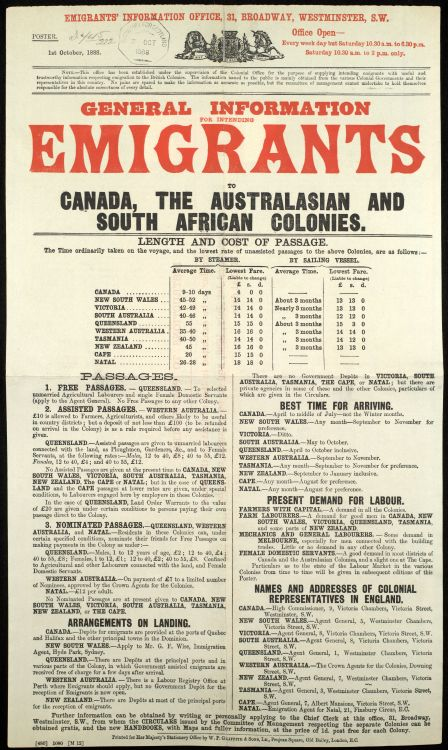
\includegraphics[scale=1.8]{img/Canadaemigration.png}
   \caption  [A Poster advertising emigration to the colonies in 1830]{ {A Poster advertising emigration to the colonies in 1830 \protect\footnotemark} } 
   \end{wrapfigure} 
 \footnotetext{source: \url{http://www.educationscotland.gov.uk/marksonthelandscape/curriculum/citizenship/migration.asp}} 
 
 It is human nature to want to seek out and to improve the manner in which we live, as is evidenced throughout human history. Humans have constantly emigrated from one country or region to another, seeking a better way of life or a better environment. The different motivations behind these emigrations include better employment opportunities, freedom, political or religious rights, famine, drought, disease, poverty, expulsion by armed force, coercion, natural disasters, better educational opportunities, or even better medical facilities.  In today’s day and age, humans attempt to improve their lives in ways other than simply moving in hope of a better life, looking to the use of additional or alternative technologies as a primary example.
 \newpage
 In this chapter, the motivations of individuals, organizations, and companies involved in the migration to the use of FLOSS will be reviewed, including, but not limited to: public collaboration, reliability, auditability, cost, security, stability, support and accountability, and flexibility and freedom (independence). The benefits of FLOSS, when compared with CSS, are far greater than they originally appear, and while cost is one of the primary motivating factors, the concept of features versus quality and the associated ease of maintenance are other major considerations. Studies have shown that many web servers have attempted to compete with and overcome the benefits of Apache, but were ultimately considered failures as a result of the tactics that were utilized on those other web servers. In fact, there is a particular network practice that allows web servers and browsers to compete in terms of which has the better features or best quality as opposed to just the different tactics; benefits are classified into three types: technical benefits, social benefits, and economic benefits.
 Figure ~\ref{fig:Motivations}  shows a diagram of some of the motivation for using the FLOSS 

  \begin{figure}
  \centering
      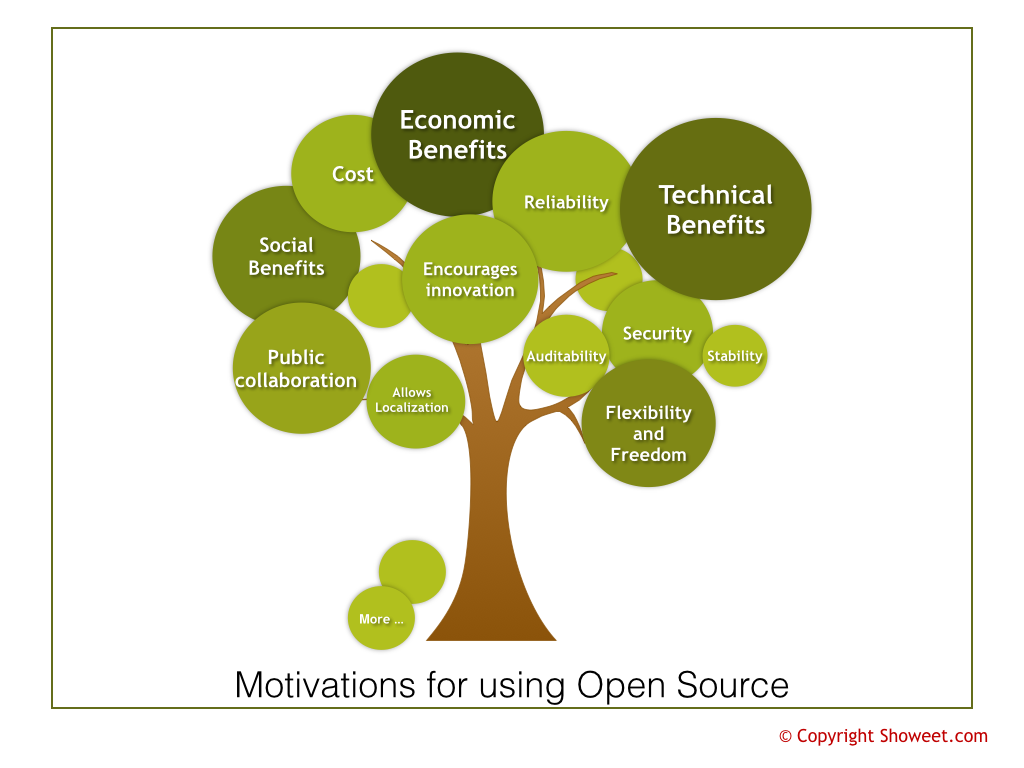
\includegraphics[scale=0.6,angle=90]{img/motivation.png}
    \caption{Motivations for using FLOSS)}
    \label{fig:Motivations}
  \end{figure}

 \section{Technical  Benefits}
 Technical benefits refer to the reliability, auditability, security, stability, allowance of localization, flexibility, freedom, support, and accountability of a given software, all of which play a vital role in the decision to migrate to FLOSS.


 \subsection {Reliability}
 \textit{ "The general business case for open-source is reliability. Open-source software is peer- reviewed software; it is more reliable than closed, proprietary software. Mature open-source code is as reliable as software ever gets."}
  Eric Raymond \footnote{\url{http://bat8.inria.fr/~lang/hotlist/free/licence/raymond/open-economics.html}}

 According to Standard Glossary of Software Engineering Terminology\footnote{ \url {http://dis.unal.edu.co/~icasta/ggs/Documentos/Normas/610-12-1990.pdf}} software reliability is defined as \textit{“The ability of a system or component to perform its required functions under stated conditions for a specified period of time”.}

 This mean Reliability refers to whether or not the developed software is free of defects relating to data error and/or loss, incorrect operations, or sudden failures. In utilizing FLOSS, many defects that do end up being found are able to be fixed within mere hours of detection, and the maintenance and update processes are quite simple for individuals and software developers alike. FLOSS has an overall value robustness given the fact that it is embedded with reliable standards, ensuring that not only is the product able to hit the market in its earliest stages, but is highly robust when this occurs. FLOSS promotes quality and reliability through the support of the rapid evolution of the source code and independent peer reviews, two aspects that are missing when dealing with CSS.


 \subsection{Security }
 Since the source code in FLOSS is open, defects and security flaws are more easily found.	Security may seem to be an advantage and a disadvantage at the same time. FLOSS allows its users to access the source code, editing, modifying, and changing the code, which results in potential vulnerabilities, yet it allows all those with access to the code to search and correct those vulnerabilities, quickly and easily rectifying those issues. The transparency offered by FLOSS becomes its greatest asset in this case; while no software is ever fully secure, the amount of transparency offered by FLOSS ensures that it is more secure than other options. It was found that issues were found and corrected quicker in FLOSS than they were in any CSS options. It was revealed that FLOSS had a lower defect density than that of CSS.
 	According to Evans Data Corporation Survey\footnote{Spring 2002 Linux Developer Survey.Wheeler David A. Available at \url{http://www.osepa.eu/site\_pages/News/43/WhyOSS\_Look\_at \_the\_numbers\_Wheeler\_2007.pdf}} reports that Linux systems are relatively immune from attacks as security breaches are rare in Linux Environment. 78\% of the respondents to the GNU/Linux developers’ survey have never experienced an unwanted intrusion and 94\% have operated virus-free. The survey shows that GNU/Linux “doesn’t get broken into very often and is even less frequently targeted by viruses,”
 	
 	These qualities are the reason for the appearance of open source products in response to security requirements. For example, \ac{NSA} in United states released a Linux kernel security module known as \ac{SELinux} which provides the mechanism for supporting access control security policies, including the Department of Defense.
   \subsection {Auditability}
   
   Is a factor at the time the source code gets published. Cross verification of the code with  CSS indicates that FLOSS is far better than CSS as the CSS forces the end user to trust that the vendor and/or developer has worked to ensure that there are no backdoors, that the program is secure, and that there is a flexibility for future modification of the program and adherence to basic security standards. If the developers will not fix the problem, the user has the option of fixing it or hiring someone else to fix it. 
   
   As the source code is not available for CSS, this type of trust cannot be verified by an independent source, with CSS options that this trust is not always founded. FLOSS offers increased levels of confidence on the part of the end user that such issues do not exist by offering this increased accountability.
 \begin{figure}[H]
 	\centering
 	   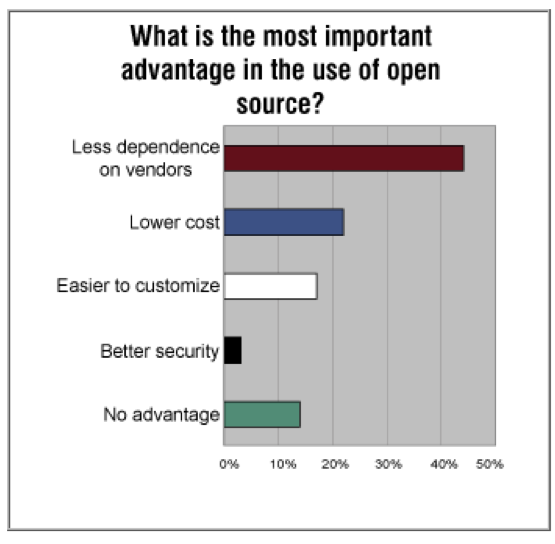
\includegraphics[width=0.6\textwidth]{img/OSSadv.png}
 	  \caption[Advantages of FLOSS]{Advantages of FLOSS (Computer Economics, Inc., 2005) \protect\footnotemark }  
 	  \label{fig:OSSsdv}
 	 	\end{figure}
 	\footnotetext{Source: \url{http://www.computereconomics.com/article.cfm?id=1043} \label{adv}}
 Figure ~\ref{fig:OSSsdv} shows the results of a survey  by "Computer Economics" about the advantages in the use of FLOSS, \textit{"The survey indicates that IT decision makers value (reduced dependence on software vendors) as the most important advantage of open source.  This indicates that software buyers must feel some level of dependence on proprietary software vendors, from which they desire freedom.  Such dependence includes reliance on the vendor for maintenance and support and the necessity for the buyer to accept version upgrades that the buyer may not need or want."}\footnote{Look at previous footnote \ref{adv}} and it also indicating how heavily cost plays a factor in preference.

 \subsection {Flexibility and Freedom } 
  The primary benefit of FLOSS adaptation is the variation that is offered. The flexibility and freedom offered by the implementation of FLOSS by a user or organization is that it facilitates changes, customization, experimentation, and offers freedom of choice to the individual or entity. When implementing CSS, users have to install set applications and files associated with that software, while the installation of FLOSS offers end users with a reliable flexibility of infrastructure, allowing the user to select the applications that they wish to install and utilize out of existing open source options. CSS has a lock in feature that requires the user to input access keys, typically paid for by the user, in order to be able to gain access to certain applications, while in FLOSS all users are able to access all applications, providing further flexibility through freedom. 

  With proprietary software the user is completely dependent on the developer . The developer may be a programmer, but may not have the necessary intimate knowledge of the field to create the best software design for the business. They are in the business of developing software, and may not be as familiar with the needs of the end user as in-house developers. FLOSS allows the company to begin with their needs and then custom design a system that is suited or it, rather than picking something of the shelf that is close, but not an exact fit. 

  \subsection {Stability} 

  Other factors that make users more likely to switch over to FLOSS include the concept of a standard format and increased stability. In utilizing FLOSS, the likelihood of documentation of the different formats is high, whereas in CSS  this is not always an option. The adaptation of FLOSS is more likely by end users as a result, because not only they are able to obtain an application that may be modified and potentially has been modified to meet their needs, as opposed to one that cannot be modified, but that there will likewise be documentation available regarding those modifications. 

  FLOSS allow the user to ensure that the stored data remains readable in the long term, as when using a proprietary format there is the issue that once the format becomes obsolete, the data is, in effect, lost. As many public entities are required to maintain data for decades, the use of FLOSS offers a significant advantage.

  While software vendors and developers are able to discover new ways to retain their customers or end Auditability users, the decision to migrate from one operating system or program to another still resides in the hands of the end user. The primary issue with this is that the average software user does not see this as a choice open to them, believing they have little control over the process and potentially feeling isolated and out of their league, finding this too technical for them, resulting in potential issues for themselves and their business.
 
  \subsection{Allows Localization }
   Localization occurs when the software adapts to the local language for the coding and implementation processes. Source code is often presented in the developer’s primary language; for instance if the developer is from Spain, the source code is likely to be in Spanish, and if they are from China, it is likely to be in Chinese. For other types of software this could cause an issue in problem resolution if the individual attempting to resolve the problem does not speak the primary language, however in FLOSS, there is an option for clients and end users to adapt to their localization, allowing them to obtain the source code in their primary language, allowing users to choose and modify language according to their preferences, a concept quite popular in areas where English is not the primary language.

  \textbf{The Importance of Localization} \footnote{Acording to the study "Free/Open Source Software: Localization" \url{http://akgul.bilkent.edu.tr/iosn/foss-l10n.pdf}} "
 \textit{\begin{itemize}
 \item 	Reduced reliance on imports.
 \item	Local programmers gain expertise and experience.
 \item	Local control over software appearance and functionality.
 \item  New local technical standards and educational opportunities.
 \item Establishment of a local software industry. It is difficult for foreigners to do localization as they do not normally have an intuitive feel for the local language and therefore the language is compromised in most cases.
 \item National policy on local content would not be dependant on the availability of proprietary software or hardware. 
 \item Localization of applications can be prioritized according to the national needs.
 \item Significantly reduces the amount of training necessary to empower end-users to use a computer system.
 \item Facilitates the decentralization of data at provincial and district levels. The same applies to utility companies (electricity, water, telephone), who will develop local language databases, thereby reducing costs and giving better service to citizens.
 \item Helps universities train more software engineers. "
 \end{itemize}}
%------------------------------------------------------------------
  \section{Economic Benefits}
  Economic benefits consist of cost and innovation that occur when users are motivated to adopt FLOSS in their organizations or companies. The developers focus on the needs and requirements to be added to existing technologies and amend the source codes in FLOSS, enhancing the features with reliable innovations often free of cost. 
  
  \subsection {Cost}
  
  Cost is considered as a major benefit in FLOSS, especially in comparison to the costs associated with the use of CSS. Software developers collect certain fees under the guise of maintenance, updates, debugging, and so on, causing the costs of CSS to balloon beyond the original price point. While many users do not factor these into the cost of utilizing CSS, companies and organization must pay attention to these \ac{TCO}, making them more likely to see the implementation of FLOSS as a reasonable and cost efficient option. FLOSS offers a potential purchase price of zero, reduces administrative overheads, decreases the amount of accounting that needs to be done, reduces investment needed, reduces licensing fees, reduces upgrade costs, virus protection costs nothing, there is zero vulnerability in downtime and data loss, decreased chances of security breaches, decreased chance of system hacks, decreased chance of attacks, all of which, if occurring, would raise the overall system cost and administrative load. 
  
  Migration to FLOSS also eliminates corporate control of the entity. This is a key reason cited for conversion to FLOSS, particularly for government entities. Migrating to FLOSS
 not only reduces the initial costs of the software, it also reduces the \ac{TCO}. There is no initial cost of the software. There is lower administrative overhead and no need to account for the number of copies that are distributed. CSS usually only allows a certain number of issues of the software before an additional fee will occur.  
  \begin{figure}[H]
     \begin{center}
        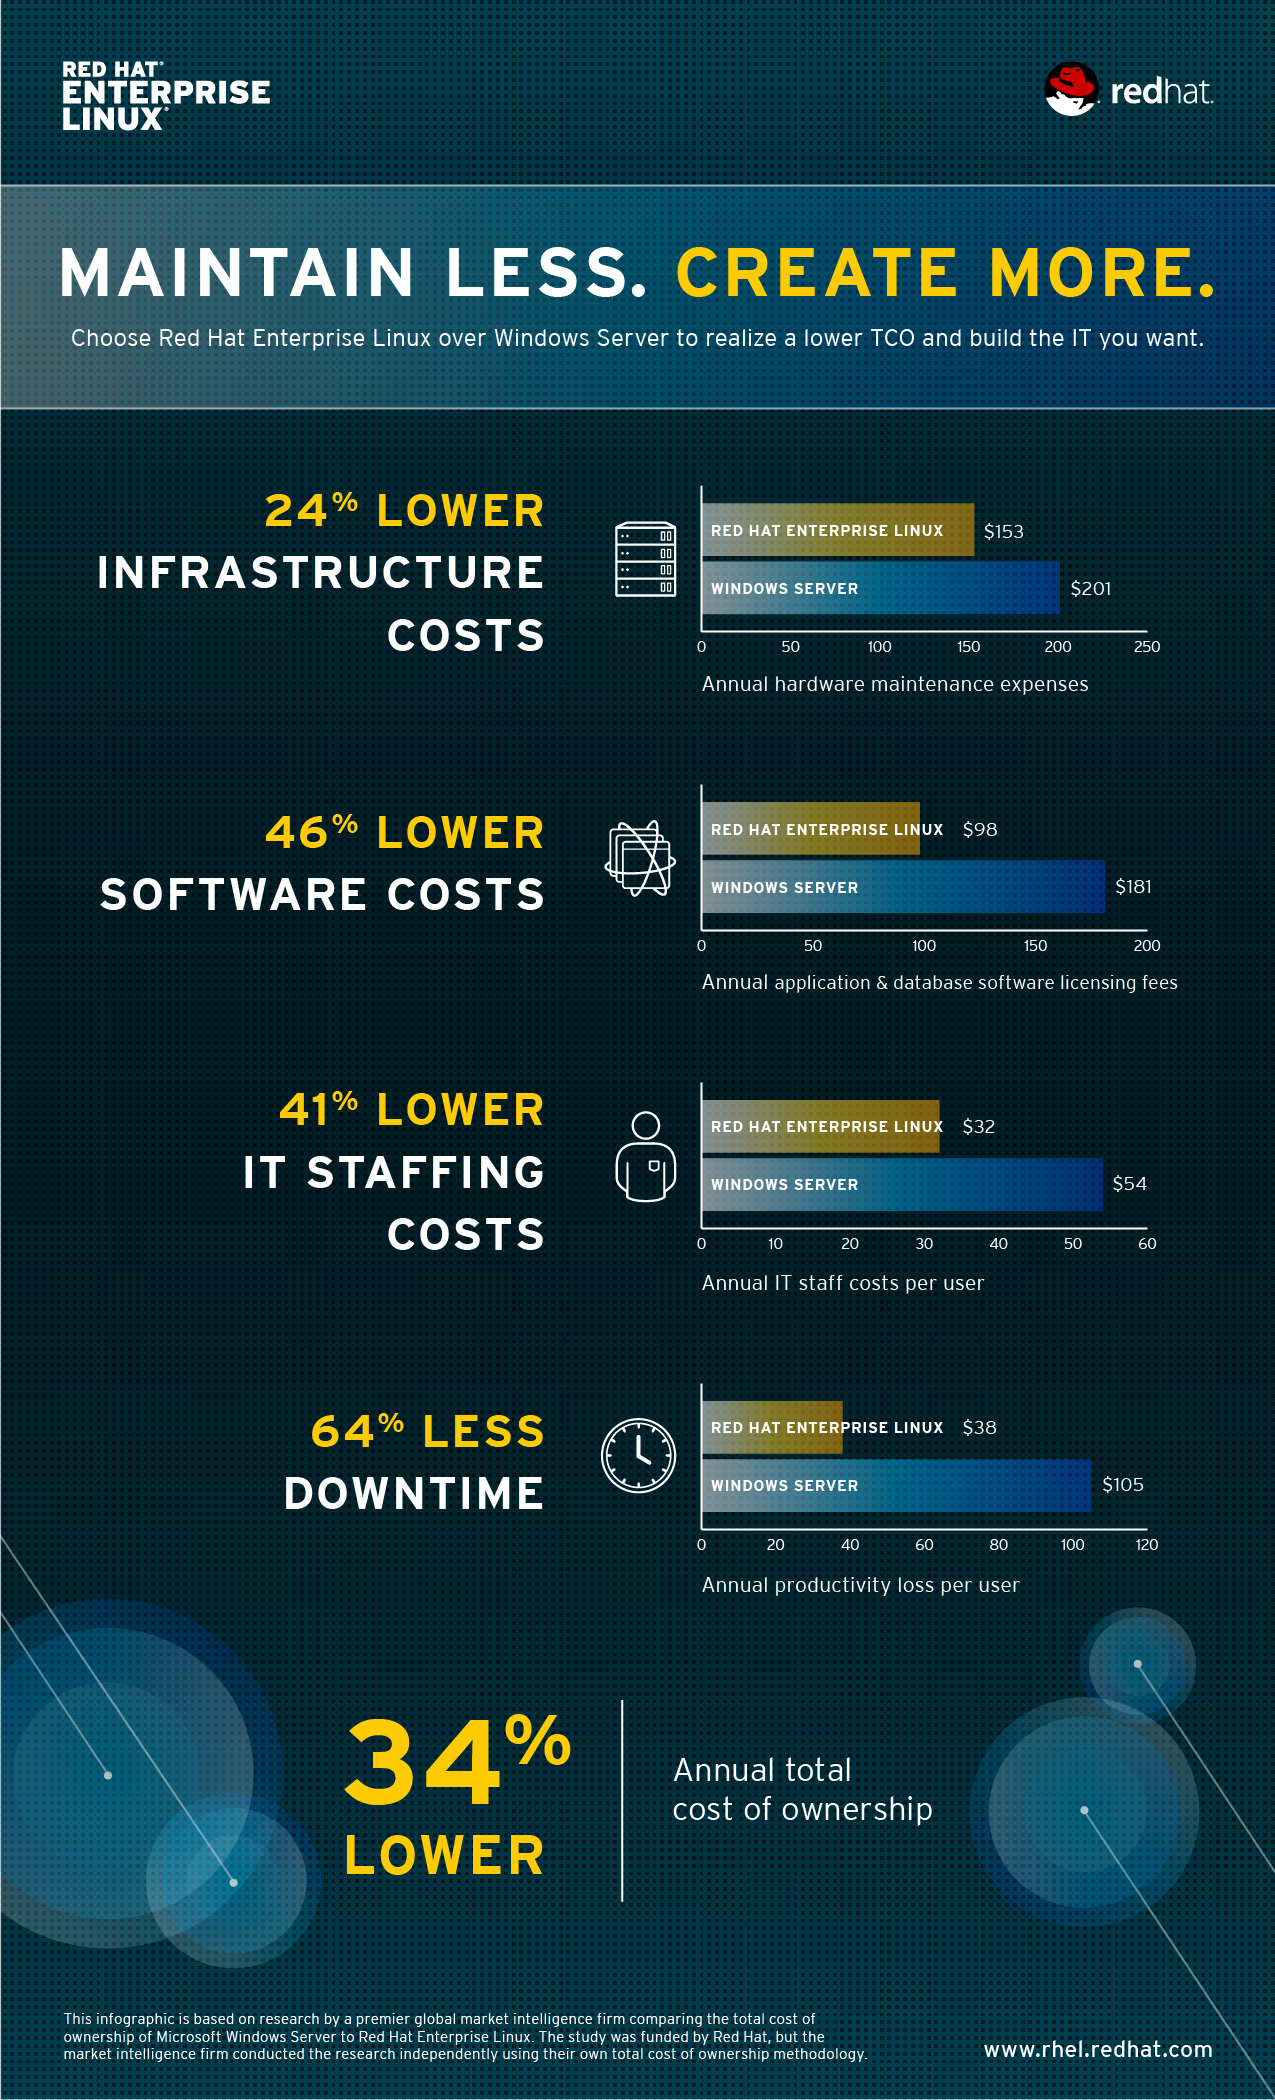
\includegraphics[scale=0.4]{img/RHELFancy.png}
       \caption[Red Hat realize lower TCO] {Red Hat Enterprise choose linux over Windows server to realize lower TCO \protect\footnotemark}
       \label{fig:RedHat}
     \end{center}
       \end{figure}
  \footnotetext{Source:\url{http://www.redhat.com/en/about/blog/how-red-hat-enterprise-linux-trims-total-cost-of-ownership-in-comparison-to-windows-server}\label{fo:redhat}}
 In a study by Red Hat, compared costs and efficiencies of two commonly deployed IT infrastructure platforms: Red Hat Enterprise Linux and Microsoft Windows Server.\textit{ " Based on expenses measured per year per user, the study recorded significant annual savings for Red Hat Enterprise Linux versus Windows in three cost categories: server infrastructure costs (29\% lower), IT staffing costs (41\% lower), and costs from lost user productivity (64\% lower). Taken together, Red Hat Enterprise Linux systems provided an annual TCO savings of 34\% over Microsoft Windows."}
   \footnote{look at previous footnote  (\ref{fo:redhat})}

 
Figure ~\ref{fig:RedHat} shows how infrastructure platforms based on Red Hat Enterprise Linux experienced the TCO  to 34\% lower annual TCO per user compared to systems running Windows Server.

 \subsection{Encourages innovation}
  The use of FLOSS offers an increased chance of innovation, which increases the overall value of the software itself. In the combination of cost, reliability, and innovation, FLOSS ends up outperforming CSS  each time.
  The innovations in the technology have impacted the FLOSS users to generate plans and motivate the FLOSS developers to enhance the current technology with up-gradation. The innovative technologies in the ICT development around the world have attracted several users to adopt the FLOSS instead of staying with the CSS. For instance, in the study conducted by(Zhussupova and Rahman) \footnote{Zhussupova .A and Rahman .A.A., (2011), “Open Source Software Adoption in Public Organizations of Kazakhstan”, Journal of IEEE: Conference on Open Systems, 7(1), 417\-502,2012, Elsevier.} the organizations in Kazakhstan and Malaysia, shifted from their traditional licensed based technologies and adopted the FLOSS in order to get better results. Other studies that have proved the intense use of FLOSS in biometrics and aeronautics and space have also proved that the results attained by the researches in their study with the help of FLOSS was reliable than that of the results that were attained with the help of CSS. The innovative technologies in the field of education adapted themselves to the FLOSS platforms where the staffs at the universities and the libraries can utilize the exploratory design of the software where the training is unnecessary and the support of the communities was approachable. Since there are no particular ways to seek support directly from the software developer in order to clarify the doubts in the FLOSS products, the users encouraged the developers to come up with innovative technologies where they can seek help from other developers or users in the community or the developer himself would provide solutions by creating his own community, thus both the users and the developers would be benefited. Allowing for all to adjust the software, as their imagination lets them.  
  
  \section{Social Benefits }
  The social structure that is created by FLOSS encourages programmers to become users, and vice-versa, as this allows the users and the programmers alike to understand the needs of the other. The most natural relationship that occurs is one that is directly reciprocal between the two. Programmers write the software for the users, and the users suggest features to programmers and report bugs when they are found, allowing for a closer and more mutually beneficial relationship between the two.
  
  While the social and societal value of FLOSS is not always highlighted by either the public or the private sector, it results in the unfettered sharing of knowledge, increases the formulation of rules, and works to redefine methods of data manipulation and procedures. Knowledge works to ensure that a better future may be shaped from the current state of economics and as a result of the productivity of the situation. Opinion leaders and experts often advocate to their customers that knowledge should be equally shared and spread around the globe and within society as freely and widely as possible.
  
  \subsection{Public collaboration}
  Public collaboration is one of the major factor that benefits the organizations and the businesses with the FLOSS implementation. Behind each and every projects, several programmers focus specially on collaborating to generate and improve a flawless website with better framework. Though there are several companies that makes use of proprietary or workstations or home built systems as their website frameworks which were created by themselves, there are companies that make use of the FLOSS like Drupal and WordPress which were developed through the talents of thousands of developers. Thus the public would be motivated by the FLOSS preferred by the companies rather than using the CSS.
  \newpage
  
  It may be inferred from the above identified benefits that FLOSS is: cost free, license fee free, user friendly, reliable, auditable, a public collaborative, securable, stable, supportable, accountable, flexible, and independent, enable localization of software to native languages, faster technology development through collaborative innovation and development of the domestic IT industry, generate opportunities in the form of more and better jobs, by learning and training more personal growth opportunities. better businesses, better government by more efficient institutions, and reduction of dependence on monopolistic CSS vendors.
  
  The FLOSS being zero cost provides faster ways in adapting to the technologies in organization than that of the proprietary software and also provides the companies with license free models such as service based models deviating from the traditional models. The adoption of FLOSS is quite easier and faster and the software provides the end users with ease of access and synchronization.
  
  As a result using FLOSS is a reasonable or even better compared to CSS. This result is also supported by studies by various research, but benefits offered depend largely on context, with the benefits remaining higher when compared with CSS. The key factors that makes FLOSS more reliable are that developers are usually also users of the software, developers are members of a community of developers, public availability of the source code and fast bug removal practices since thousands of independent programmers testing and fixing bugs of the software.
